% Document type with options
\documentclass[fleqn,letterpaper,12pt]{report}

% Required packages and settings (DO NOT UPDATE THIS)
\usepackage{UN5390}
../LaTeXTemplates/Course/UN5390_Settings.tex

% Assignment-specific setting (UPDATE THIS WHEN NECESSARY)
\week{04}

% Document begins
\begin{document}

% Title (DO NOT UPDATE THIS)
\assignmenttitle

%
\phantomsection
\addcontentsline{toc}{section}{Problem \# 1}
\problem
{\bf Red Flags Rule }\\
The Red Flags Rule requires many businesses and organizations to implement a written Identity Theft Prevention Program designed to detect the warning signs – or red flags – of identity theft in their day-to-day operations.The bottom line is that a program can help businesses spot suspicious patterns and prevent the costly consequences of identity theft.The Federal Trade Commission (FTC) enforces the Red Flags Rule with several other agencies.This article has tips for organizations under FTC jurisdiction to determine whether they need to design an identity theft prevention program.\cite{RF}\\
\\
{\bf Federal Information Security Modernization Act (FISMA)}\\
The Federal Information Security Modernization Act (FISMA) of 2014 updates the Federal Government's cybersecurity practices. It does it by Codifying Department of Homeland Security (DHS) authority to administer the implementation of information security policies for non-national security federal Executive Branch systems, including providing technical assistance and deploying technologies to such systems. It also 
Amends and clarifies the Office of Management and Budget's (OMB) oversight authority over federal agency information security practices; and by requiring OMB to amend or revise OMB A-130 to eliminate inefficient and wasteful reporting.\cite{FIMA}\\
\\
{\bf Family Educational Rights and Privacy Act (FERPA)}\\
The Family Educational Rights and Privacy Act (FERPA) (20 U.S.C. § 1232g; 34 CFR Part 99) is a Federal law that protects the privacy of student education records. The law applies to all schools that receive funds under an applicable program of the U.S. Department of Education.FERPA gives parents certain rights with respect to their children's education records. These rights transfer to the student when he or she reaches the age of 18 or attends a school beyond the high school level. Students to whom the rights have transferred are "eligible students."\cite{FE}




%
\newpage
\phantomsection
\addcontentsline{toc}{section}{Problem \# 2}
\problem
The Psuedo-code is the code for generating Prime numbers upto the number {\bf d}. The Outer loop increments values upto d and each time the inner loop divides the value d by the numbers upto a. 

The number of floating point operations can be mathematically given as $$y = 0.5*d^2 + 0.5*d ;$$
where {\bf y} is the number of floating point operations.

This method can be further improved by reducing the number of floating point operations. If we reduce the iterations to half on the inner loop , it will still produce the same output. That is each number is being divided by the numbers that span half of its size. 

The program for the calculation of the number of floating point operations is in the {\em problem2.m} file.
%
\newpage
\phantomsection
\addcontentsline{toc}{section}{Problem \# 3}
\problem
Machine epsilon ia the maximum relative error of the chosen rounding procedure. According to IEEE 754-2008 standard the machine epsilon given by  $ b^{-(p-1)} $ ,where 'p' is the precison. Therefore for a single precision 32 bit binary where 1 bit is implicit, epsilon is $ 2^{-23} $ and a 64 bit binary it is $ 2^{-52} $.

The program for the calculation of the Machine epsilon is in the {\em machine\_epsilon.m} file.
\begin{figure}[ht!]
	\centering
	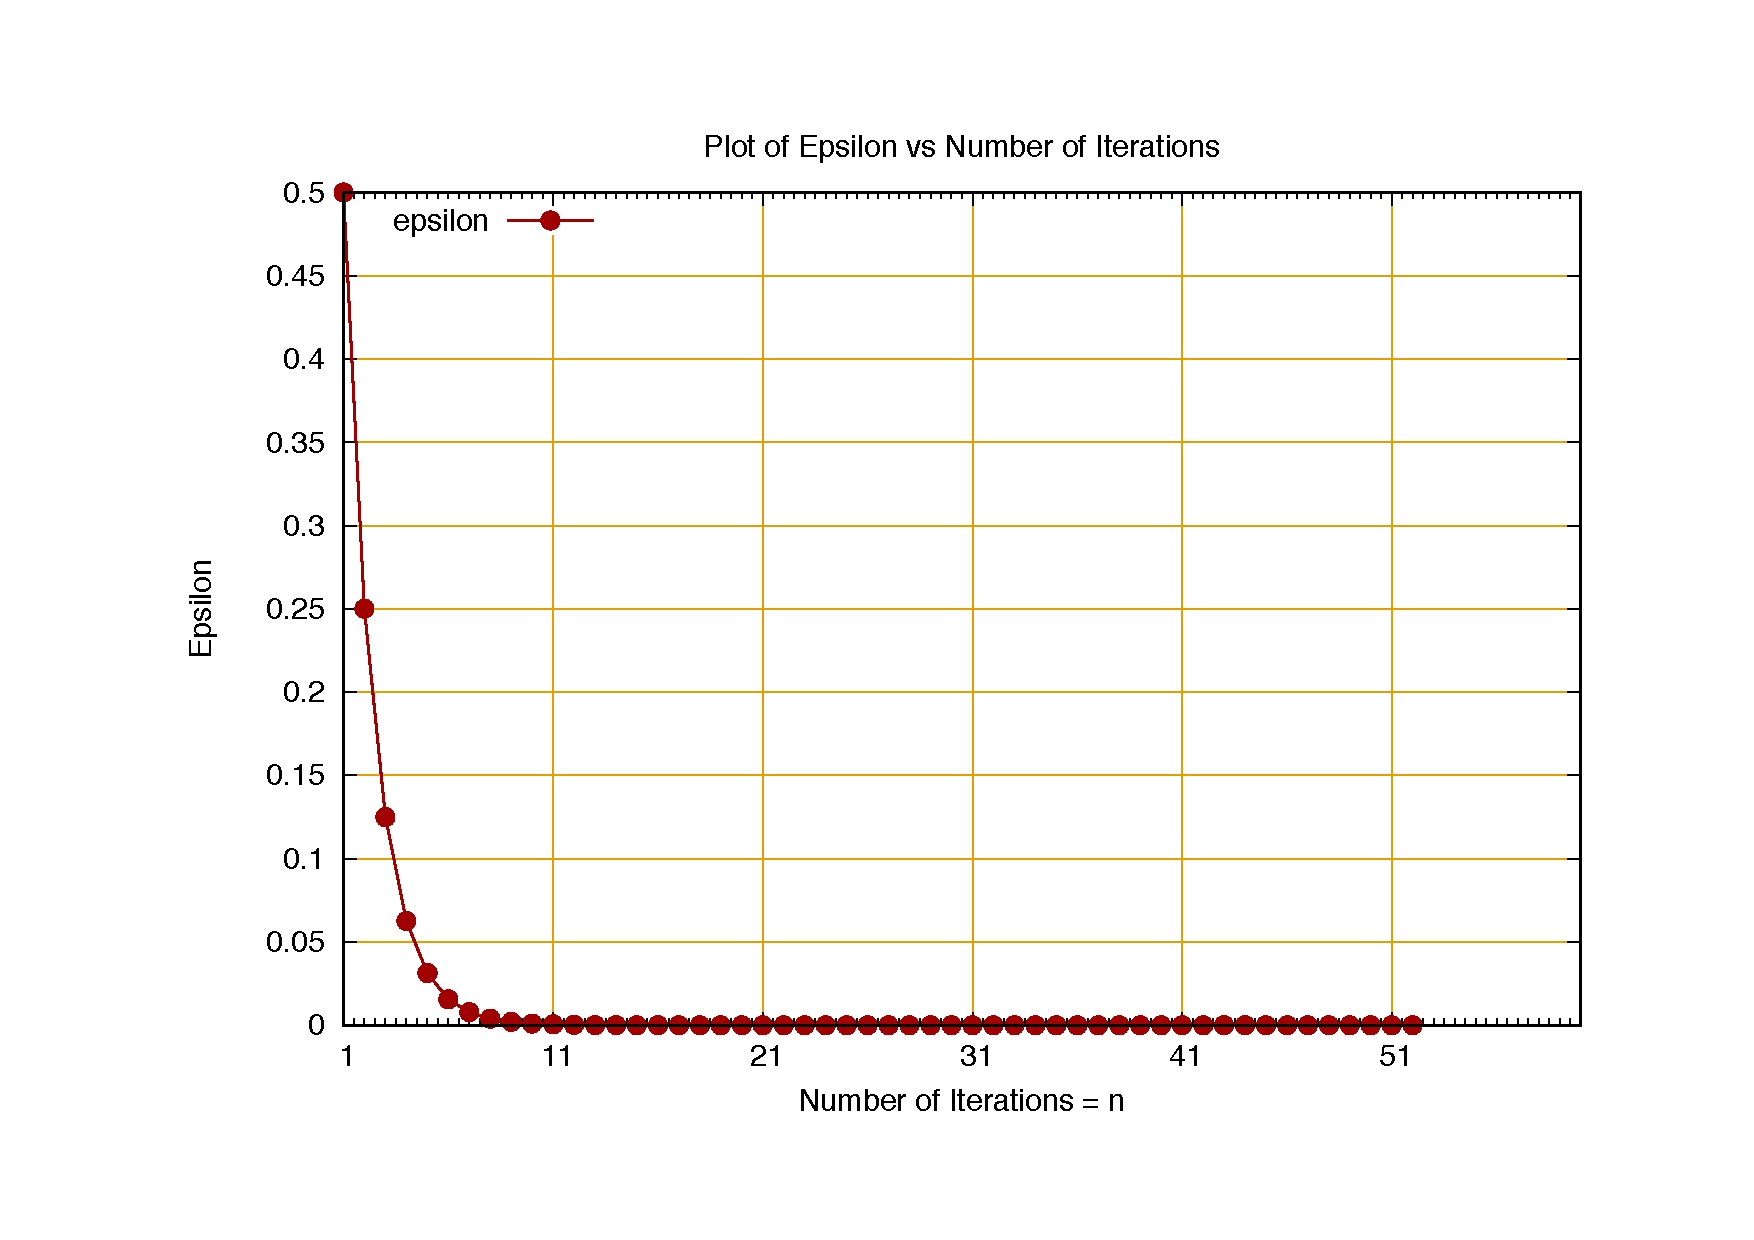
\includegraphics[height=120mm,width=160mm]{machine_epsilon.pdf}
	\caption{Epsilon vs Number of Iterations n\label{overflow}}
\end{figure}

%
\newpage
\phantomsection
\addcontentsline{toc}{section}{Problem \# 4}
\problem
The Approximation for Eulers constant {\bf \em e} is performed using the two expressions given. The main difference between the two approximations is that the first approach is discrete which means that that the values are calculated on discrete integers which means this is an approximation. The second approach is usual approach to calculate $ e^x$. It is caluated for all the values on the number line. The second approach is more accurate and is the right way to do it. This will only be an approximation if n is not considered to be infinity.

The program for the calculation of the Eulers constant is in the {\em exp\_x.m} file.
%

\newpage
\phantomsection
\addcontentsline{toc}{section}{Problem \# 5}
\problem
The Probabilty of getting exactly {\em h} heads in {\em n} tosses is given by, for a coin with probabilty {\em  P} 
$$ P(h\ heads\ exactly) = \binom{n}{h}.p^h.(1-p)^{(n-h)} $$
,where {\bf p} is the probabilty that the coin is fair or the fairness factor. 

For 7 heads in 10 trails, we have,
$$ P(7\ heads\ exactly) = \binom{10}{7}.p^7.(1-p)^{(n-h)} $$

For a fair coin $ p=0.5$, Hence,
$$ P(7\ heads\ exactly) = 120*0.5^7*(1-0.5)^3 $$
$$ P(7\ heads\ exactly) = 0.1172 $$

A fair coin theoritically from above has 0.1172 chance of getting 7 heads in 10 tosses. It cannot be said, therefore, with certainity said that the coin is fair or not fair because for 7 heads to show up in a consequetive 10 tosses the coin it can be the outcome of a fair coin with the probabilty of the outcome being 0.1172. 

From a therotical perspective, the Probabilty that the coin is fair can be inferred after multiple experiments of the tossing of coins for different n's and depending on the number of heads/tails we consider the P(p) to some calculated value(which depends on the experiments). This is called Bayesian inference.  
$$ P(p/h) = {{\binom{n}{h}.p^h.(1-p)^{(n-h)}}*p(h)}/P(p) $$
\clearpage
\begin{figure}[ht!]
	\centering
	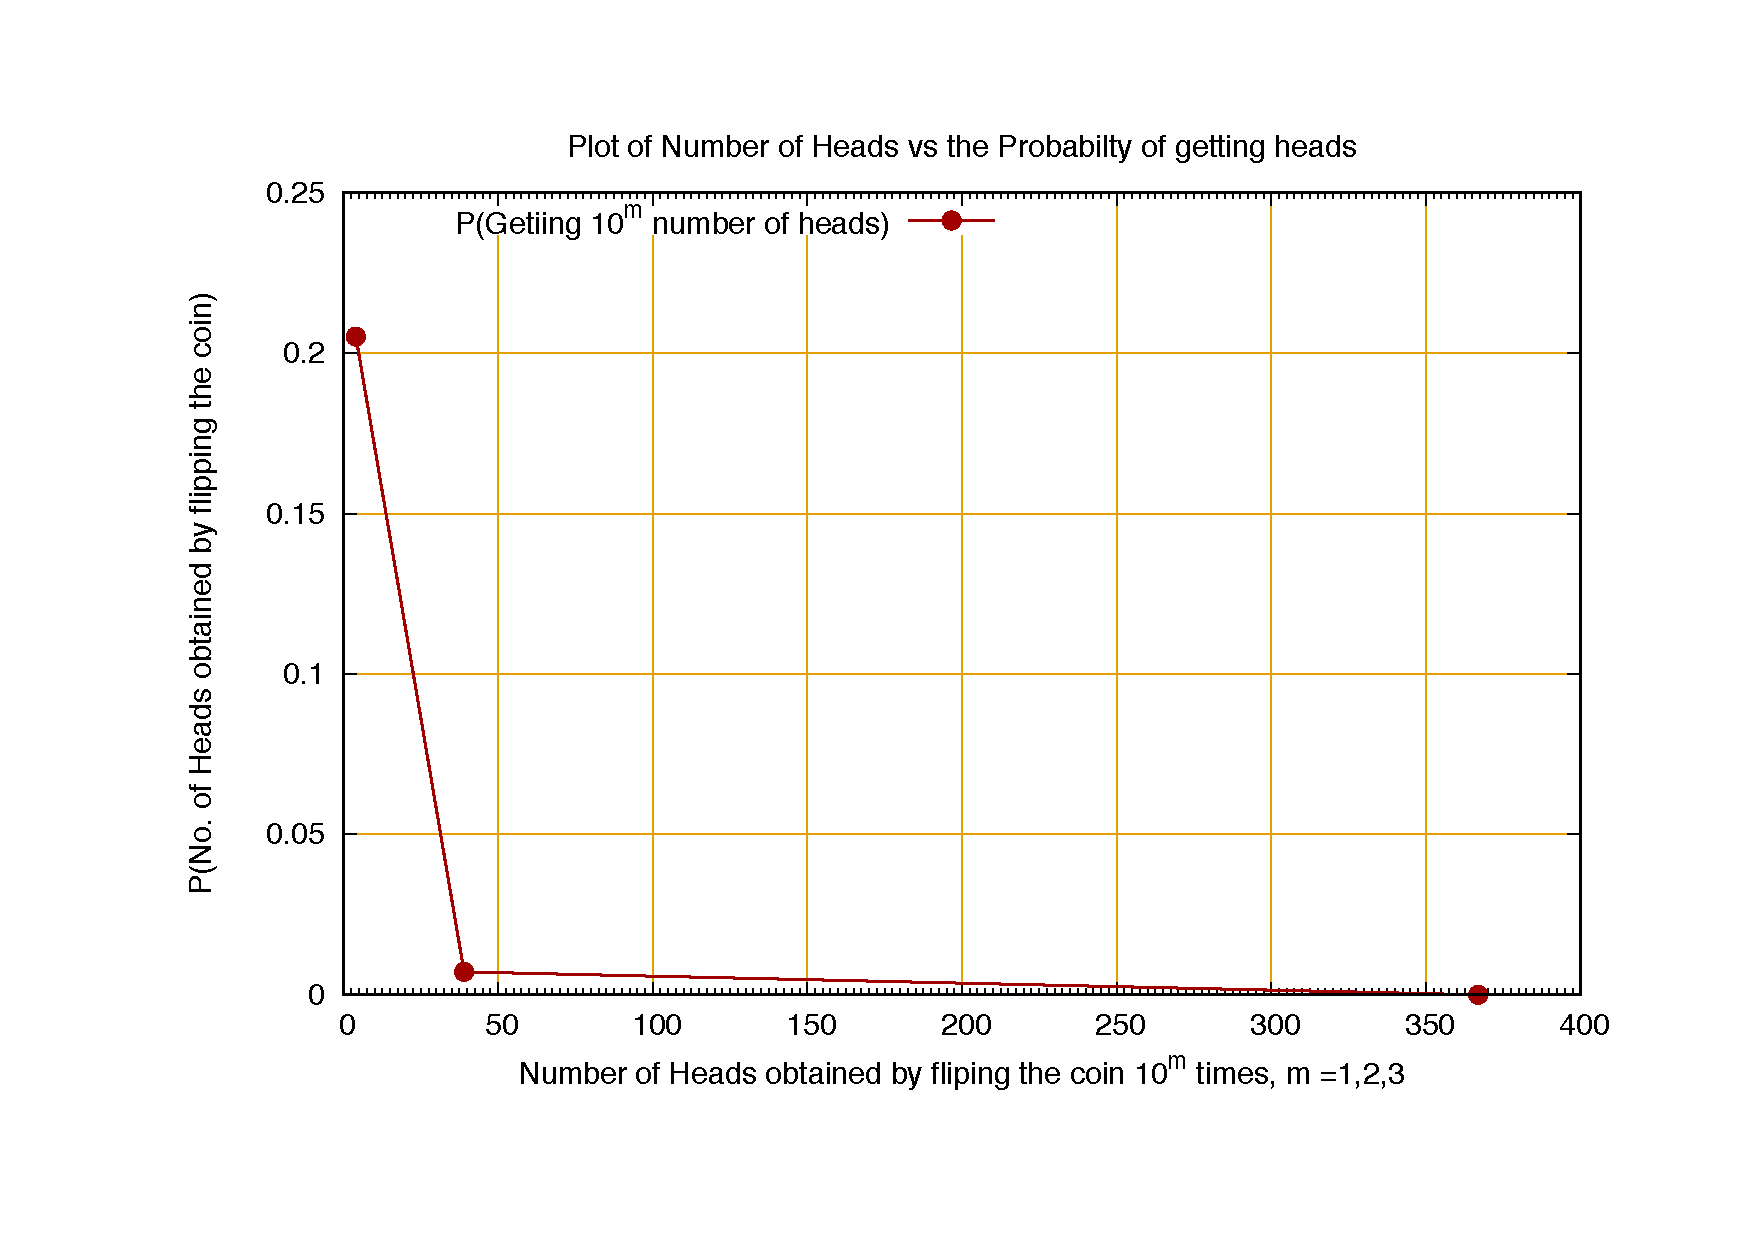
\includegraphics[height=140mm,width=140mm]{CoinFlip_single.pdf}\caption{The figure shows that as we increase the number of tosses, the probabilty of getting a certain number of heads decreases. 
 \label{overflow}}
\end{figure}
\clearpage

\begin{figure}[ht!]
	\centering
	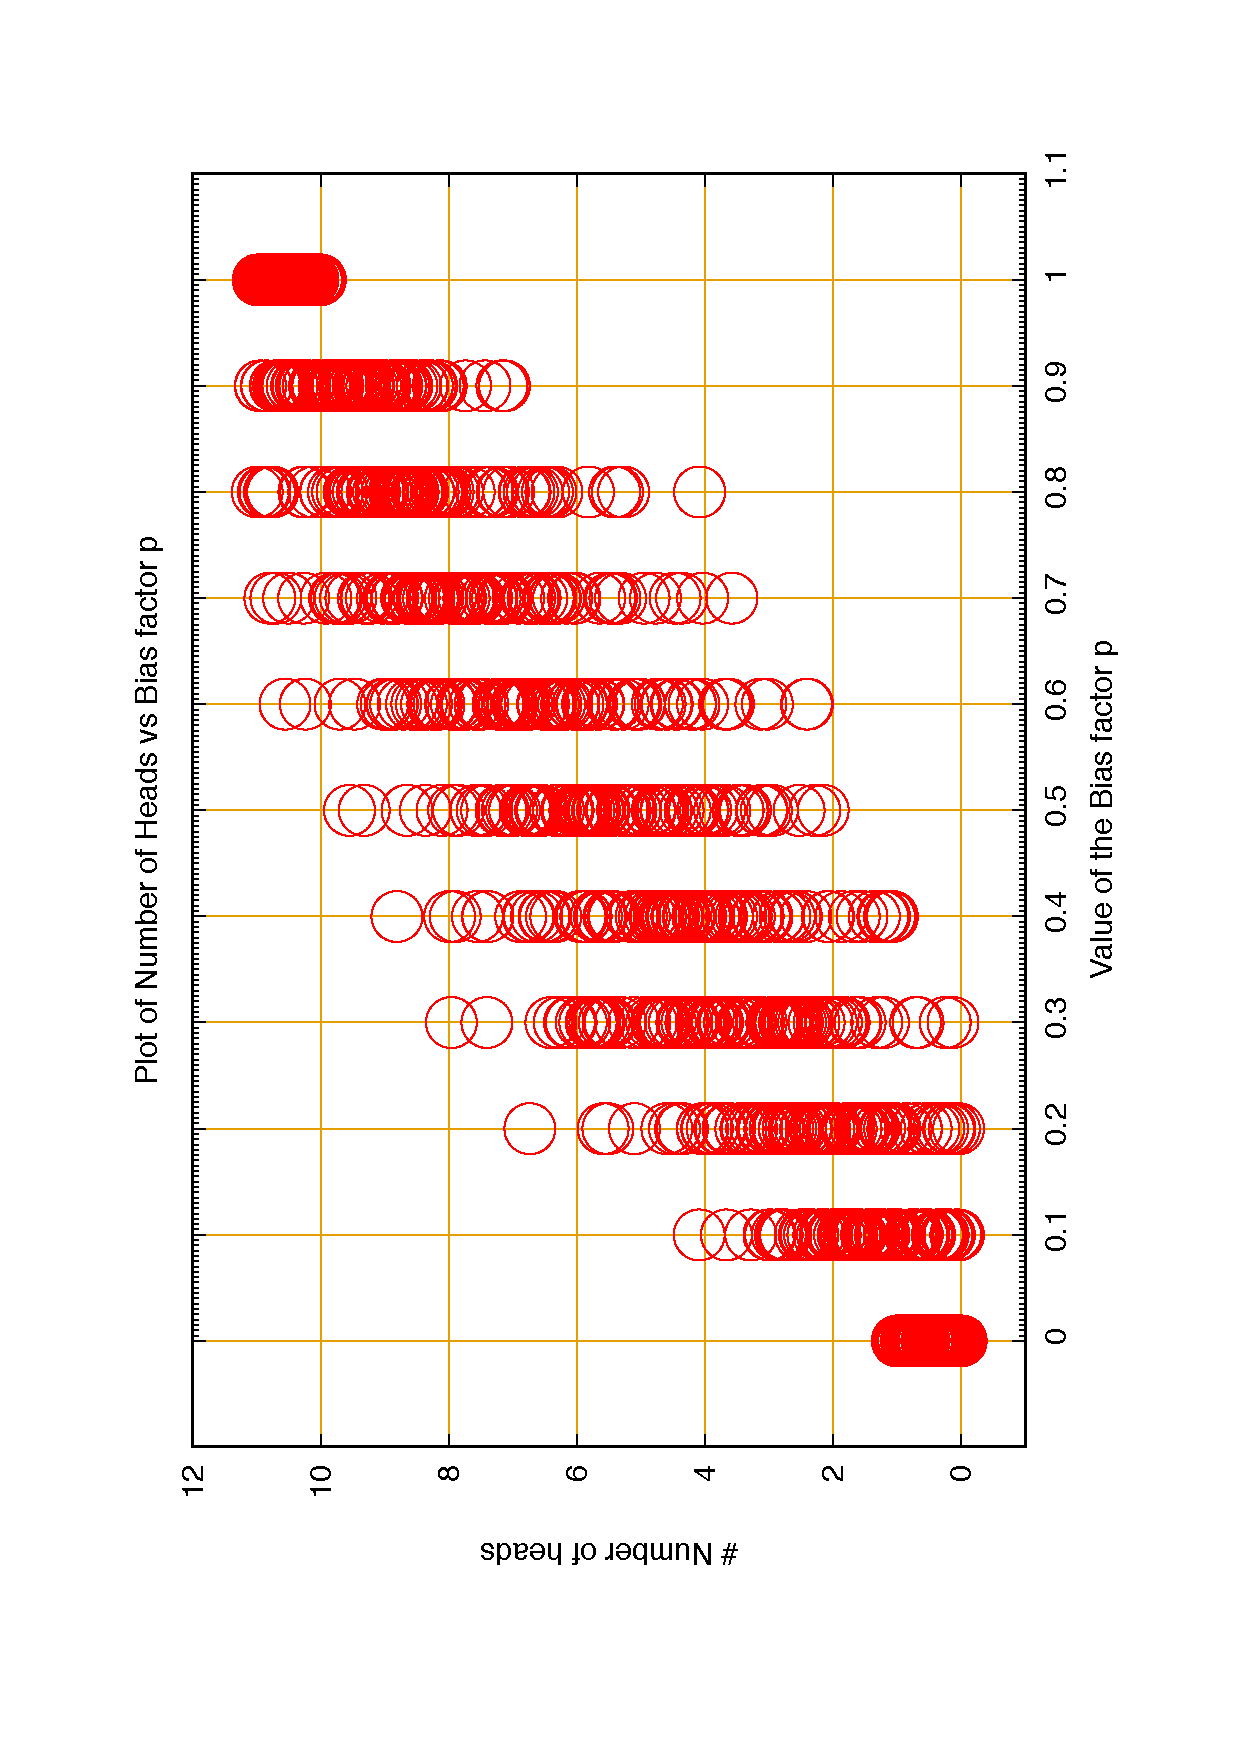
\includegraphics[height=160mm,width=120mm,angle=-90]{CoinFlip_Multiple.pdf}\caption{As there is increase in the bias the majority of the results fall according to the bias. for e.g. If the bias factor is either "0" or "1", the number of heads are close to zero or one. 
 \label{overflow}}
\end{figure} 
\vfill
%
\newpage
\clearpage
\phantomsection
\addcontentsline{toc}{section}{Problem \# 6}
\problem

%

%
\newpage
% References
% http://tex.stackexchange.com/questions/84099/bibliographies-from-multiple-bib-files
\phantomsection
\addcontentsline{toc}{section}{References}
\section*{References}
\bibliographystyle{unsrt}
\bibliography{sgowtham,slanka} % REPLACE john WITH YOUR MICHIGAN TECH ISO USERNAME

% Document ends
\end{document}
